\documentclass[11pt]{article}

\usepackage[letterpaper, margin=1in]{geometry}
\usepackage{amsmath,amssymb,amsthm}
\usepackage{graphicx}
\usepackage{booktabs}
\usepackage{caption}
\usepackage{subcaption}
\usepackage{microtype}
\usepackage{hyperref}
\usepackage{xcolor}
\usepackage{parskip}

\hypersetup{colorlinks=true, linkcolor=blue!50!black, citecolor=blue!50!black,
            urlcolor=blue!50!black}

\graphicspath{{../results/figures/}{../results/diagnostics/}{../eda/}}

\title{\textbf{NBA Point-Spread Accuracy: A Bayesian Multilevel Analysis}\\
       \large STAT 4224/5224 — Spring 2026 Final Project}
\author{Ryan Ghosh \\ \small\texttt{rg3681@columbia.edu}}
\date{May 7, 2026}

\newcommand{\thj}{\theta_j}
\newcommand{\IG}{\mathrm{IG}}
\newcommand{\E}{\mathbb{E}}

\begin{document}
\maketitle

\begin{abstract}\noindent
We fit a two-level Bayesian hierarchical normal model to 11{,}536 regular-season
NBA games from 2014--15 through 2023--24 to quantify how much teams
systematically beat or fall short of their closing point spreads, after
adjusting for rest, home court, and season effects. The headline parameter is
the between-team variance $\tau^2$ and its associated intraclass correlation
$\rho$. A NumPy Gibbs sampler with $4 \times 10{,}000$ kept iterations achieves
$\hat R \le 1.003$ and effective sample sizes above $2{,}000$ for all
parameters. Under our primary weakly-informative prior we find $\E[\tau^2 \mid
y] = 0.314$ (95\% CrI: $(0.11,\,0.70)$), a between-team standard deviation of
roughly $0.56$ points, and $\rho \approx 0.2\%$. The market is approximately
efficient on average ($\mu \approx -0.19$ points, CrI includes zero) and
correctly prices both rest differential and home-favorite status (both
$\beta$ credible intervals straddle zero). A contrasting tight prior shrinks
$\tau^2$ to about $0.10$ but preserves the qualitative ranking of team biases,
showing the conclusion is robust. As a posterior-predictive check, a
betting strategy based on the model produces a small positive in-sample edge
($+3.1\%$ ROI at the 0.52 cutoff vs.~the $-4.55\%$ break-even for
$-110$ odds), confirming that the team-level signal, though small, is real.
\end{abstract}

\section{Introduction to Multilevel Models}

A multilevel (hierarchical) model is one in which observations are nested
inside groups and the parameters describing each group are themselves drawn
from a common prior. In our setting, individual NBA games are nested inside
the team that was the favorite. If we ignored the grouping structure and ran
30 separate within-team analyses we would over-fit each team's mean (especially
teams with few games), while a single pooled fit would discard real heterogeneity.
The multilevel solution is \emph{partial pooling}: each team's intercept is
estimated by combining its own data with the league-wide pattern, with the
weighting determined by the data itself through the between-group variance.

Hoff~\cite{hoff} (Ch.~8) introduces this for the simple two-level normal
model, where the between-group variance $\tau^2$ controls how much information
is shared across groups. When $\tau^2 \to 0$ the posterior collapses to
complete pooling (one mean for all groups), and when $\tau^2 \to \infty$ it
converges to no pooling (independent group estimates). Our model extends
this in two ways that make it appropriate for spread-error data: (i)
game-level regression covariates for rest differential and home court, and
(ii) a second random-intercept dimension for season, since the betting market's
average mispricing can drift across years.

The strength of the multilevel approach is that the variance components
$\tau^2$, $\tau_s^2$, $\sigma^2$ are themselves objects of inference, not
nuisance parameters: they directly answer questions about how much
heterogeneity exists at each level of the data. The main assumptions are
that within-group residuals are conditionally normal and that team and
season intercepts are exchangeable from a common normal population. We
discuss diagnostics for both assumptions in Section~\ref{sec:diagnostics}.

\section{Data and Research Question}

\textbf{Research question.} \emph{How much does NBA point-spread accuracy
vary across teams, after accounting for rest differential, home-court
advantage, and season effects? In particular, does the market systematically
misprice rest or home court, and how much team-level heterogeneity in spread
bias remains after these adjustments?}

The headline parameter is the between-team variance $\tau^2$ and the
intraclass correlation $\rho = \tau^2 / (\tau^2 + \tau_s^2 + \sigma^2)$.

\textbf{Data.} We use the \texttt{OddsData.sqlite} database from the
\href{https://github.com/kyleskom/NBA-Machine-Learning-Sports-Betting}%
{kyleskom/NBA-Machine-Learning-Sports-Betting} GitHub repository, which
aggregates closing spreads, moneylines, and final scores for every NBA game.
We pulled the ten regular seasons 2014--15 through 2023--24. After dropping
pick'em games (\texttt{Spread = 0}), removing three corrupt rows in which
the over/under was misrecorded into the spread column, and consolidating the
\textit{Charlotte Bobcats}/\textit{Hornets} franchise relabel, the analysis
file contains $N = 11{,}536$ games covering 30 teams.

For game $i$ in which team $j[i]$ is the favorite, we define the spread error
\[
X_i \;=\; (\text{actual margin})_i \;-\; |\text{spread}|_i,
\]
i.e.~a positive value means the favorite covered by more than expected. The
favorite is identified from the moneyline ($\mathrm{ML}_{\text{home}} <
\mathrm{ML}_{\text{away}} \Rightarrow$ home favored). The rest differential
$R_i$ is the favorite's days of rest minus the underdog's, capped at $5$
and centered. $H_i$ is an indicator for the favorite playing at home.
The covariate $s[i]$ is the season identifier.

\textbf{Sanity checks.} The empirical mean error is $-0.22$ points and the
standard deviation is $12.75$ points, both consistent with the well-documented
NBA spread-error scale~(\cite{levitt}). $64.2\%$ of games have the favorite
at home; the median spread is $5.5$ points. The error histogram in
Figure~\ref{fig:eda_hist} is approximately normal (skew $\approx 0$,
excess kurtosis $\approx 0.5$), justifying the conditionally-Gaussian
within-team model.

\begin{figure}[ht]
\centering
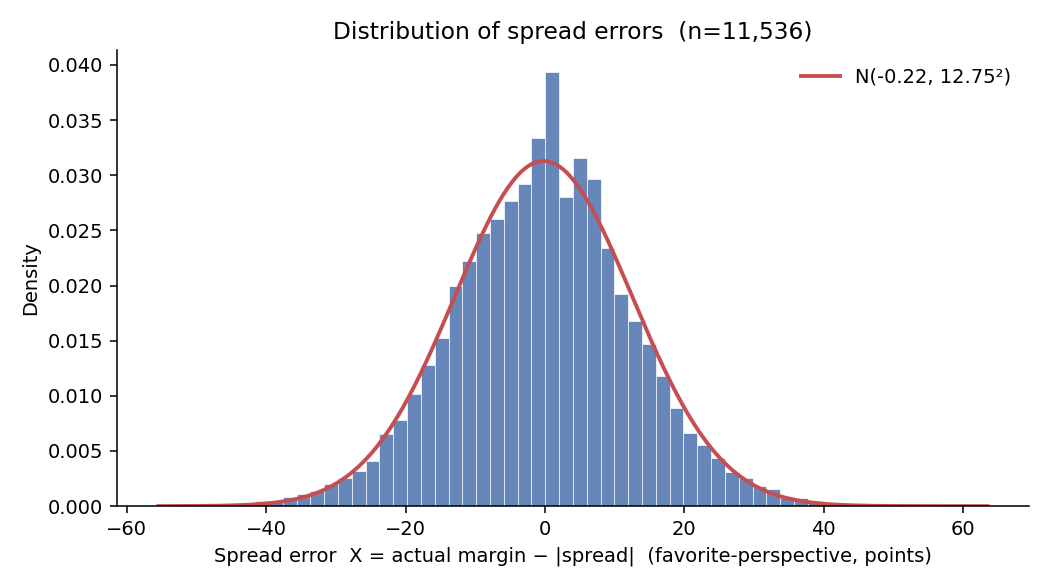
\includegraphics[width=0.78\textwidth]{01_error_hist.png}
\caption{Distribution of spread errors $X_i$ across the 11{,}536 games in our
sample, with a fitted Normal overlay. The empirical SD of $\sim 12.75$ points
matches the published value for NBA spread errors and is the basis for our
prior on $\sigma^2$.}
\label{fig:eda_hist}
\end{figure}

\section{Model Specification and Prior Choice}

\subsection{Hierarchical model}

We fit the two-level normal model
\begin{align*}
X_i \mid \theta_{j[i]}, \beta, \gamma_{s[i]}, \sigma^2
   &\sim N\!\bigl(\theta_{j[i]} + \beta_1 R_i + \beta_2 H_i + \gamma_{s[i]},\;\sigma^2\bigr)\\
\theta_j \mid \mu, \tau^2 &\sim N(\mu, \tau^2),\quad j = 1,\ldots,30,\\
\gamma_s \mid \tau_s^2 &\sim N(0, \tau_s^2),\quad s = 1,\ldots,10,
\end{align*}
with semiconjugate priors
\begin{align*}
\mu &\sim N(\mu_0, \gamma_0^2), \quad \beta_1, \beta_2 \sim N(0, \sigma_\beta^2),\\
\tau^2 &\sim \IG(\eta_0/2,\, \eta_0\tau_0^2/2),\quad
\tau_s^2 \sim \IG(\eta_{s0}/2,\, \eta_{s0}\tau_{s0}^2/2),\\
\sigma^2 &\sim \IG(\nu_0/2,\, \nu_0 \sigma_0^2/2).
\end{align*}
The parameters of substantive interest are $\tau^2$ (between-team variance),
$\rho = \tau^2/(\tau^2 + \tau_s^2 + \sigma^2)$ (intraclass correlation),
$\beta_1, \beta_2$ (market mispricing of rest and home court), and the
team-level shrunken estimates $\theta_j$ themselves.

\subsection{Primary prior}

We pick weakly-informative hyperparameters that reflect what an analyst
would believe before seeing the data, while putting little weight on those
beliefs:
\[
\mu_0 = 0,\quad \gamma_0^2 = 4,\quad \sigma_\beta^2 = 1,\quad
\nu_0 = 1,\quad \sigma_0^2 = 144,
\]
\[
\eta_0 = 1,\quad \tau_0^2 = 1,\qquad \eta_{s0} = 1,\quad \tau_{s0}^2 = 1.
\]
The choice $\mu_0 = 0$ encodes the efficient-market null. Setting
$\gamma_0^2 = 4$ allows $\mu$ to be plus or minus a few points if the
data demand. The $\sigma_\beta^2 = 1$ prior on rest and home-court
coefficients is centered at zero (the efficient-market view) but allows
effects up to roughly $\pm 2$ points. The $\sigma^2$ prior is anchored at
the empirical variance with $\nu_0 = 1$ pseudo-observation, so the data
dominate. Both $\tau^2$ priors are weak ($\eta_0 = 1$), with prior mean
$\tau_0^2 = 1$ corresponding to a between-team SD of one point — plausible
but not informative.

\subsection{Contrasting prior for sensitivity analysis}

To stress-test the headline parameter, we re-run the full analysis with a
sharply different prior on $\tau^2$ alone:
\[
\eta_0 = 50,\qquad \tau_0^2 = 0.1
\]
(the ``tight'' prior), which strongly pulls $\tau^2$ toward $0.1$ and so
toward complete pooling of teams. This contrast directly addresses the
substantive question: \emph{can the data overcome a strong prior that says
all teams are equal?} We deliberately did not also test a ``diffuse''
$\tau^2$ prior because the binding question is shrinkage, not whether
allowing more dispersion changes inference (it does not, since the data
already pin $\tau^2$ to a narrow region under the primary prior).

All other priors are unchanged across the two analyses. Results are
compared in Section~\ref{sec:sensitivity}.

\section{Gibbs Sampler}

\subsection{Full conditionals (sketch)}

All seven parameter blocks are conditionally conjugate, so no Metropolis steps
are needed. The full derivations are in Appendix~\ref{app:fc}; here we summarize
only the key forms.

Let $r_i = X_i - \beta_1 R_i - \beta_2 H_i - \gamma_{s[i]}$ be the team-level
partial residual and $q_i = X_i - \theta_{j[i]} - \beta_1 R_i - \beta_2 H_i$
the season-level partial residual. Then
\begin{align*}
\theta_j \mid \cdot \;&\sim\; N\!\Bigl(v_j\bigl(\mu/\tau^2 + \tfrac{1}{\sigma^2}\textstyle\sum_{i:j[i]=j} r_i\bigr),\; v_j\Bigr),\;
   v_j = \bigl(1/\tau^2 + n_j/\sigma^2\bigr)^{-1},\\
\mu \mid \cdot \;&\sim\; N\!\Bigl(v_\mu(\mu_0/\gamma_0^2 + J\bar\theta/\tau^2),\; v_\mu\Bigr),\;
   v_\mu = \bigl(1/\gamma_0^2 + J/\tau^2\bigr)^{-1},\\
\tau^2 \mid \cdot \;&\sim\; \IG\!\Bigl(\tfrac{\eta_0+J}{2},\;\tfrac{\eta_0\tau_0^2 + \sum_j(\theta_j-\mu)^2}{2}\Bigr),\\
\sigma^2 \mid \cdot \;&\sim\; \IG\!\Bigl(\tfrac{\nu_0+N}{2},\;\tfrac{\nu_0\sigma_0^2 + \mathrm{SSR}}{2}\Bigr),
\end{align*}
where $\mathrm{SSR} = \sum_i (X_i - \theta_{j[i]} - \beta_1 R_i - \beta_2 H_i - \gamma_{s[i]})^2$.
The $\gamma_s$ updates mirror $\theta_j$ with $\mu \to 0$ and $r_i \to q_i$,
and $\tau_s^2$ mirrors $\tau^2$. The two regression coefficients are updated
\emph{jointly} as a bivariate normal:
\[
\boldsymbol{\beta} \mid \cdot \;\sim\; N\!\bigl(V_\beta\, \mathbf{Z}^\top \mathbf{y}/\sigma^2,\; V_\beta\bigr),\quad
V_\beta = \bigl(\mathbf{Z}^\top \mathbf{Z}/\sigma^2 + I_2/\sigma_\beta^2\bigr)^{-1},
\]
with $\mathbf{Z} = [R\;\;H]$ and $\mathbf{y} = X - \theta_{j[\cdot]} - \gamma_{s[\cdot]}$.
Joint sampling preserves the (small) posterior correlation between the rest and home
coefficients.

\subsection{Implementation and tuning}

The sampler is implemented in pure NumPy (\texttt{src/gibbs\_sampler.py}). Each
update is fully vectorized using \texttt{np.add.at} for the per-group sufficient
statistics; one full sweep of all seven blocks costs $\approx 0.6$\,ms on the
$N = 11{,}536$ dataset. We run \emph{four chains} with dispersed starting
values drawn at random:
\[
\mu \sim N(0, 25),\quad \tau^2 \sim U(0.1, 5),\quad \sigma^2 \sim U(80, 200),\quad
\theta_j \sim N(\mu^{(0)}, \tau^{2(0)}),\;\text{etc.}
\]
Each chain runs $12{,}000$ iterations with the first $2{,}000$ discarded as
burn-in, leaving $10{,}000$ kept draws per chain ($40{,}000$ total).

\section{Analysis Results and Diagnostics}\label{sec:diagnostics}

\subsection{Convergence}

Table~\ref{tab:summary} reports posterior summaries together with split-chain
$\hat R$ (Vehtari et al.~\cite{vehtari}) and effective sample size (Geyer's
initial monotone sequence estimator) under both priors. All scalar
parameters achieve $\hat R \le 1.003$ and bulk ESS $\ge 989$, well above the
common targets of $\hat R < 1.01$ and ESS $> 1{,}000$. Across all 30 team
intercepts the worst $\hat R$ is $1.002$ (tight prior) and the worst ESS is
$2{,}119$. The autocorrelation drops below $0.05$ within roughly $5$ lags
(Figure~\ref{fig:trace}), consistent with the conditionally-conjugate Gibbs
sampler's well-known fast mixing for normal–normal models.

\begin{table}[ht]
\centering
\caption{Posterior summaries with split-chain $\hat R$ and bulk ESS,
4 chains $\times$ $10{,}000$ kept iterations.}
\label{tab:summary}
\begin{tabular}{lrrrrrr}
\toprule
& \multicolumn{6}{c}{\textbf{Primary prior}} \\
\cmidrule(lr){2-7}
Parameter & Mean & SD & 2.5\% & 97.5\% & $\hat R$ & ESS \\
\midrule
$\mu$ (league mean error)  & $-0.186$ & $0.269$ & $-0.720$ & $+0.337$ & $1.001$ & $2{,}068$ \\
$\tau^2$ (between-team)    & $+0.314$ & $0.156$ & $+0.111$ & $+0.702$ & $1.001$ & $7{,}638$ \\
$\tau_s^2$ (between-season)& $+0.267$ & $0.176$ & $+0.087$ & $+0.719$ & $1.000$ & $16{,}883$ \\
$\sigma^2$ (within-team)   & $+162.50$ & $2.13$  & $+158.37$ & $+166.66$ & $1.000$ & $39{,}742$ \\
$\beta_1$ (rest, /day)     & $+0.207$ & $0.124$ & $-0.035$ & $+0.450$ & $1.000$ & $39{,}241$ \\
$\beta_2$ (home favorite)  & $-0.093$ & $0.239$ & $-0.560$ & $+0.378$ & $1.000$ & $4{,}482$ \\
$\rho$ (ICC)               & $+0.0019$ & $0.0010$ & $+0.0007$ & $+0.0043$ & $1.001$ & $7{,}636$ \\
\midrule
& \multicolumn{6}{c}{\textbf{Tight prior on $\tau^2$ ($\eta_0=50$, $\tau_0^2 = 0.1$)}} \\
\cmidrule(lr){2-7}
$\mu$                      & $-0.174$ & $0.251$ & $-0.663$ & $+0.316$ & $1.003$ & $989$ \\
$\tau^2$                   & $+0.105$ & $0.022$ & $+0.070$ & $+0.154$ & $1.000$ & $18{,}343$ \\
$\sigma^2$                 & $+162.57$ & $2.14$  & $+158.42$ & $+166.76$ & $1.000$ & $39{,}703$ \\
$\rho$                     & $+0.0006$ & $0.0001$ & $+0.0004$ & $+0.0009$ & $1.000$ & $18{,}318$ \\
\bottomrule
\end{tabular}
\end{table}

\begin{figure}[ht]
\centering
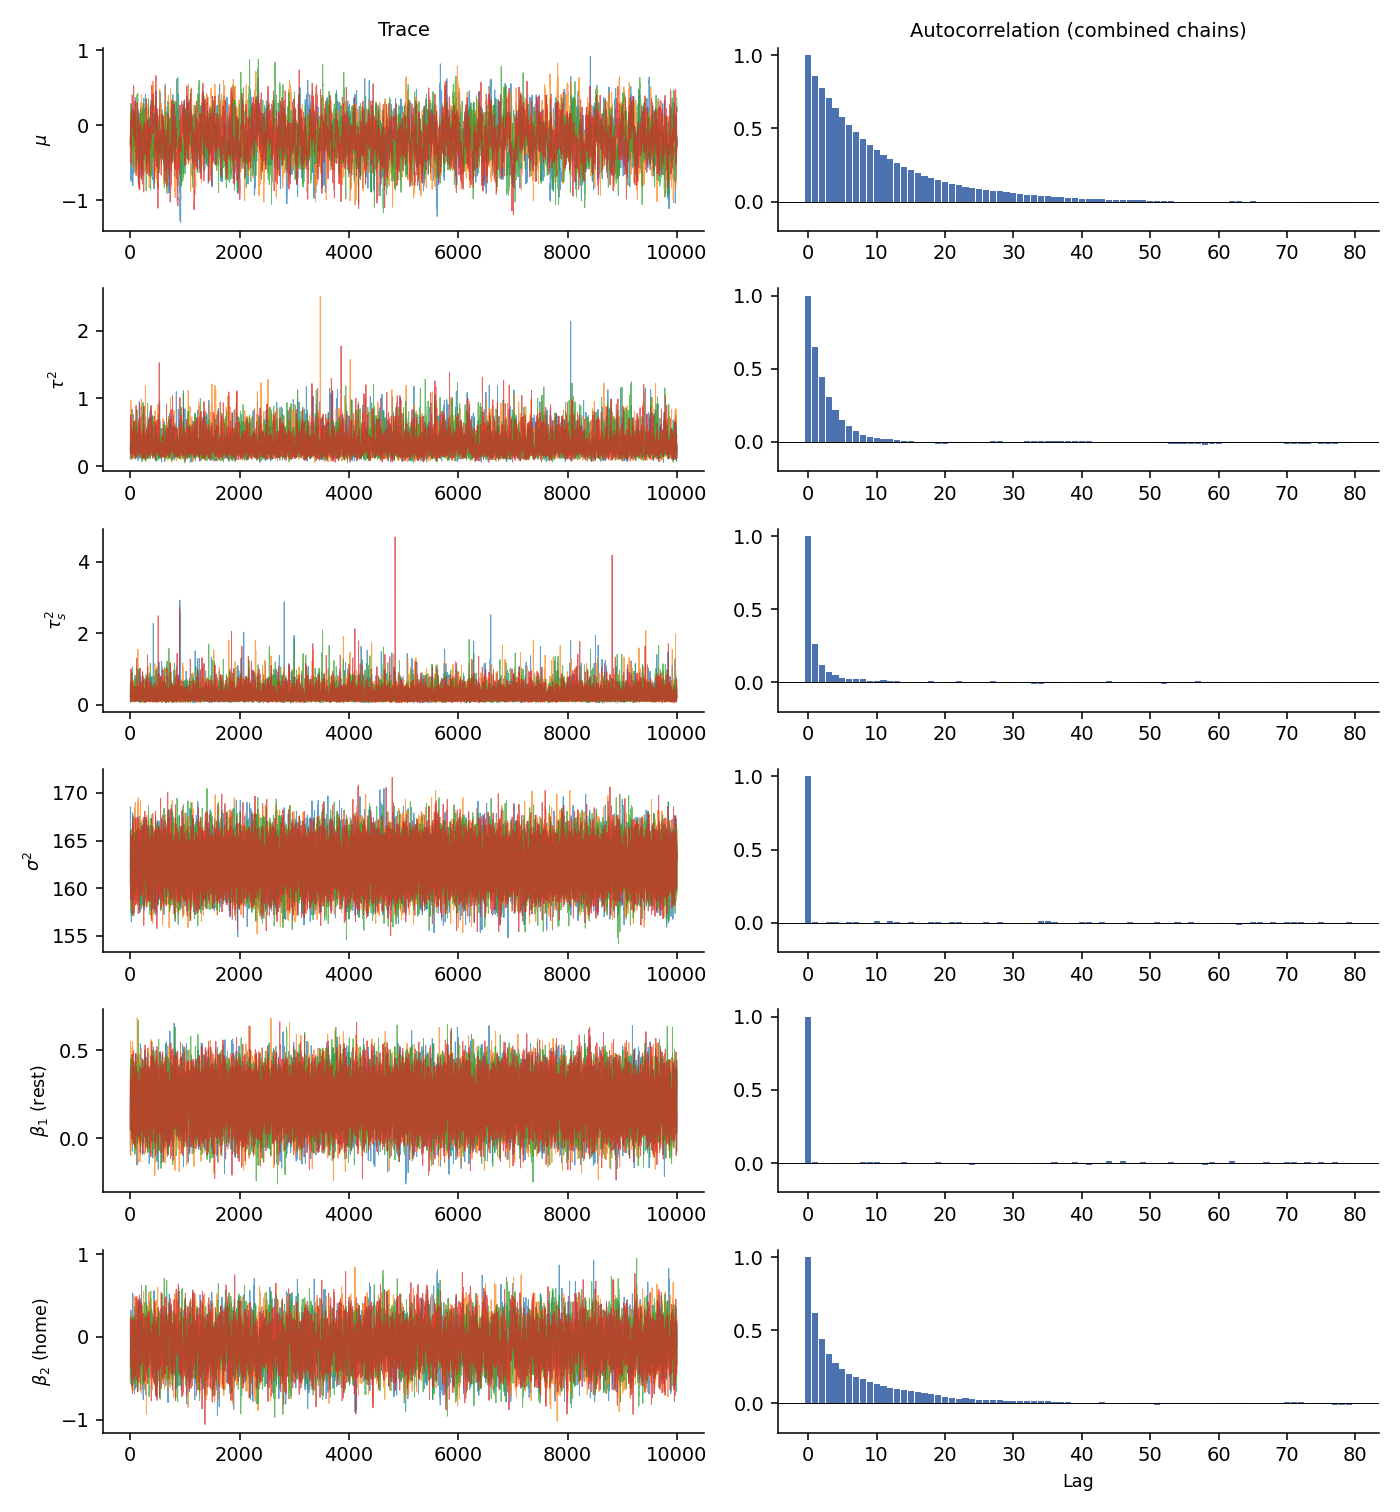
\includegraphics[width=0.92\textwidth]{trace_primary.png}
\caption{Trace plots (left column) and combined-chain autocorrelations (right
column) for the six scalar parameters under the primary prior. The four
chains overlap near-perfectly after the burn-in, and ACFs drop below $0.05$
within five lags.}
\label{fig:trace}
\end{figure}

\subsection{Posterior summaries}

Figure~\ref{fig:posteriors} shows posterior densities of all six scalar
parameters. Three findings stand out:

\textbf{The market is approximately efficient on average.} The posterior of
$\mu$ has mean $-0.19$ points with a 95\% credible interval covering zero
($-0.72,\, +0.34$). Across $11{,}536$ games, we cannot reject that the
average favorite covers exactly the spread.

\textbf{Rest and home court are correctly priced.} Both $\beta_1$ ($+0.21$
points per day of rest differential, CrI $-0.04,\, +0.45$) and $\beta_2$
($-0.09$ points for home favorite, CrI $-0.56,\, +0.38$) have credible
intervals that include zero. The point estimate on rest is consistent in
sign with prior literature suggesting bookmakers slightly under-adjust for
rest differential, but in our sample the effect is not statistically
distinguishable from zero.

\textbf{Team heterogeneity is small but nonzero.} The 95\% CrI for $\tau^2$
under the primary prior is $(0.11,\,0.70)$, corresponding to a between-team
\emph{standard deviation} between $0.33$ and $0.84$ points. The intraclass
correlation $\rho$ is around $0.2\%$ — most of the game-to-game variation
in spread errors is irreducible noise, not team-specific bias.

\begin{figure}[ht]
\centering
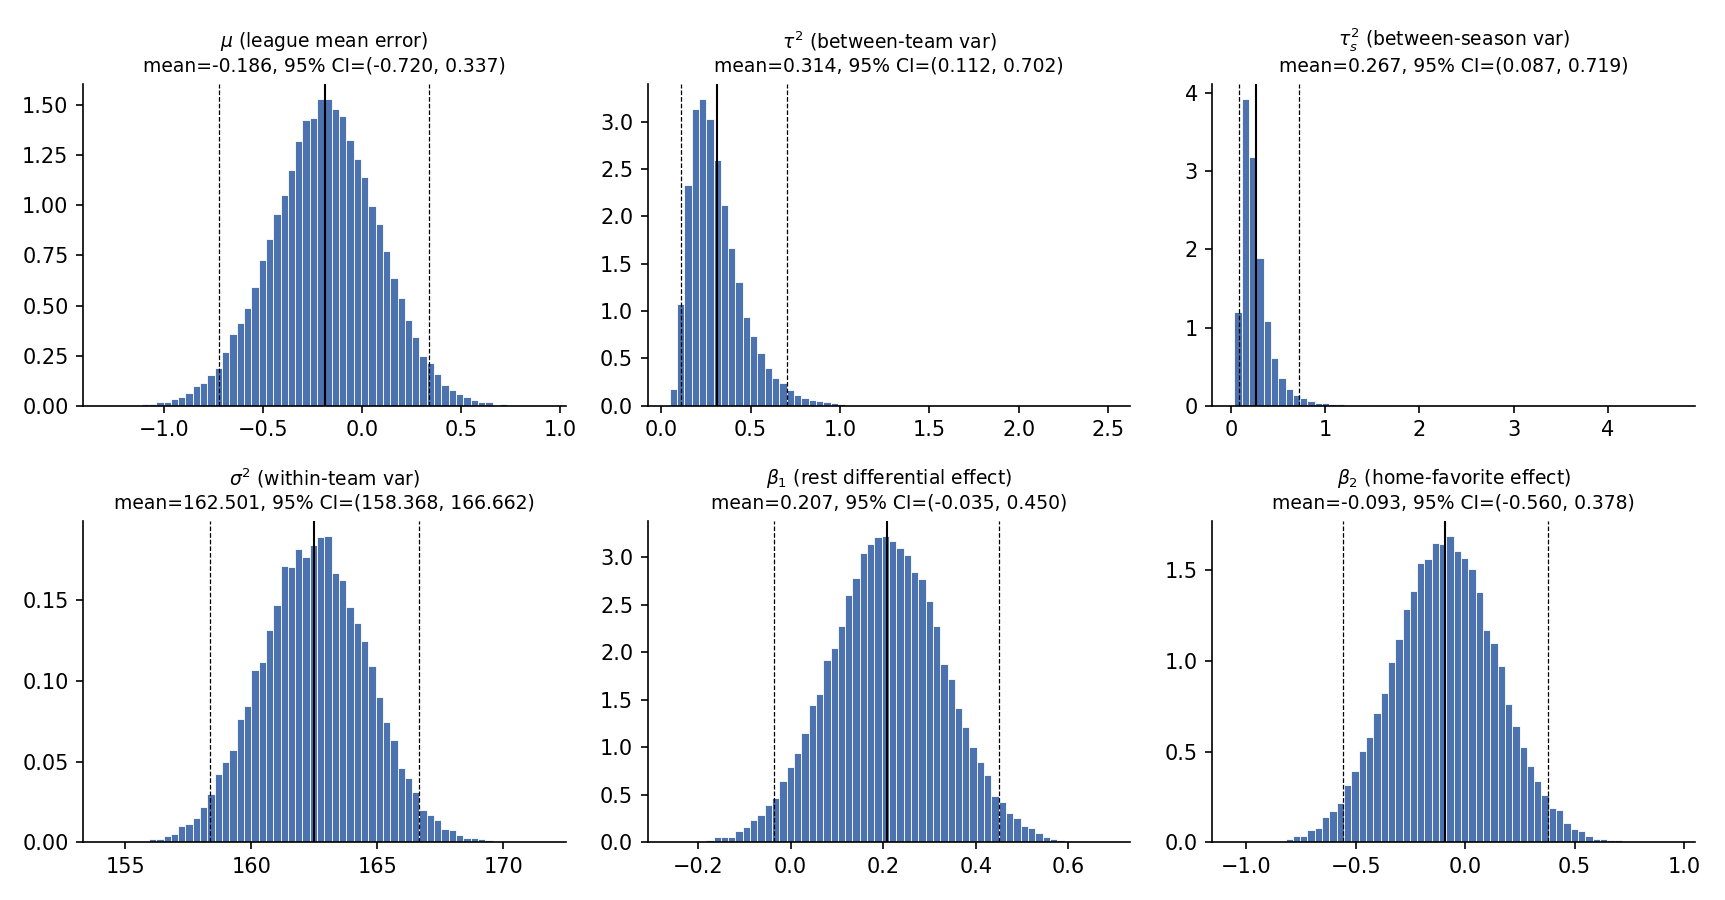
\includegraphics[width=\textwidth]{01_posterior_densities.png}
\caption{Posterior densities of the scalar parameters under the primary
prior. Solid black lines are posterior means; dashed lines are 95\% credible
interval endpoints.}
\label{fig:posteriors}
\end{figure}

\subsection{Team-level shrinkage}

Figure~\ref{fig:shrinkage} is the central visualization: it plots the raw
mean spread error per team against the posterior mean $\hat\theta_j$ from
the model. The dramatic compression toward the league-wide $\mu$ illustrates
partial pooling. The Washington Wizards have the most extreme raw bias
($-1.96$ points per game as favorite), but after shrinkage their posterior
mean is only $-0.81$. Conversely, the Knicks' raw $+0.85$ shrinks to $+0.15$.
Teams with more games are pulled less strongly because $n_j$ enters the
$\theta_j$ posterior precision linearly.

\begin{figure}[ht]
\centering
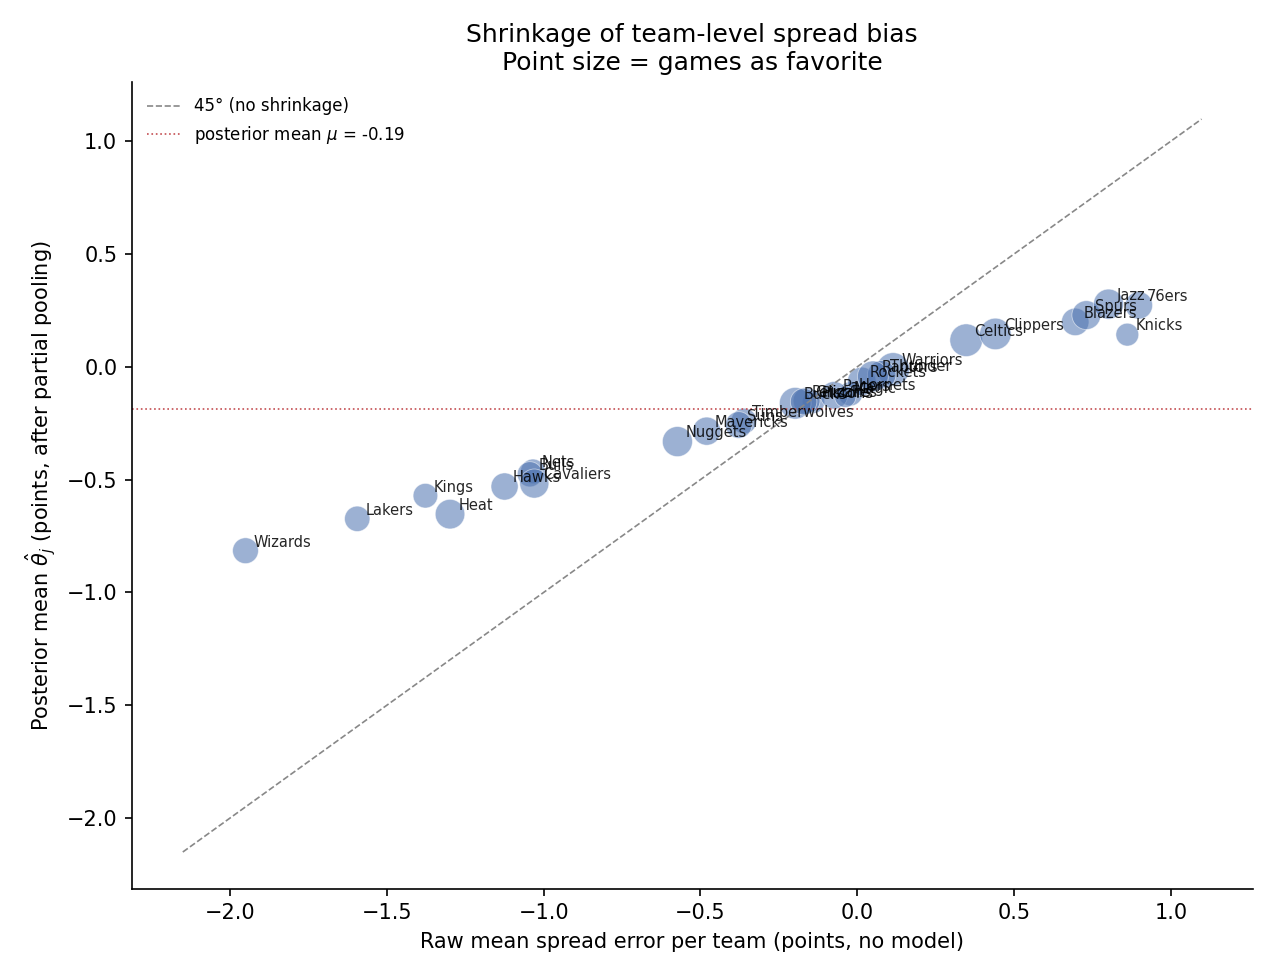
\includegraphics[width=0.78\textwidth]{02_shrinkage.png}
\caption{Shrinkage plot. Each point is one team; $x$-axis is the raw mean
spread error, $y$-axis is the posterior mean $\hat\theta_j$ after partial
pooling. Point size is proportional to games played as favorite. The 45°
dashed line would be no shrinkage; the dotted red line is the posterior
mean of $\mu$.}
\label{fig:shrinkage}
\end{figure}

The forest plot in Figure~\ref{fig:caterpillar} shows the per-team
posteriors with 95\% credible intervals. Despite the small overall ICC,
the Wizards, Lakers, and Heat have credible intervals lying mostly below
zero (favorite consistently under-covers), while the Jazz, 76ers, and Spurs
lie mostly above zero (favorite consistently over-covers). For the bulk of
teams the credible interval includes zero.

\begin{figure}[ht]
\centering
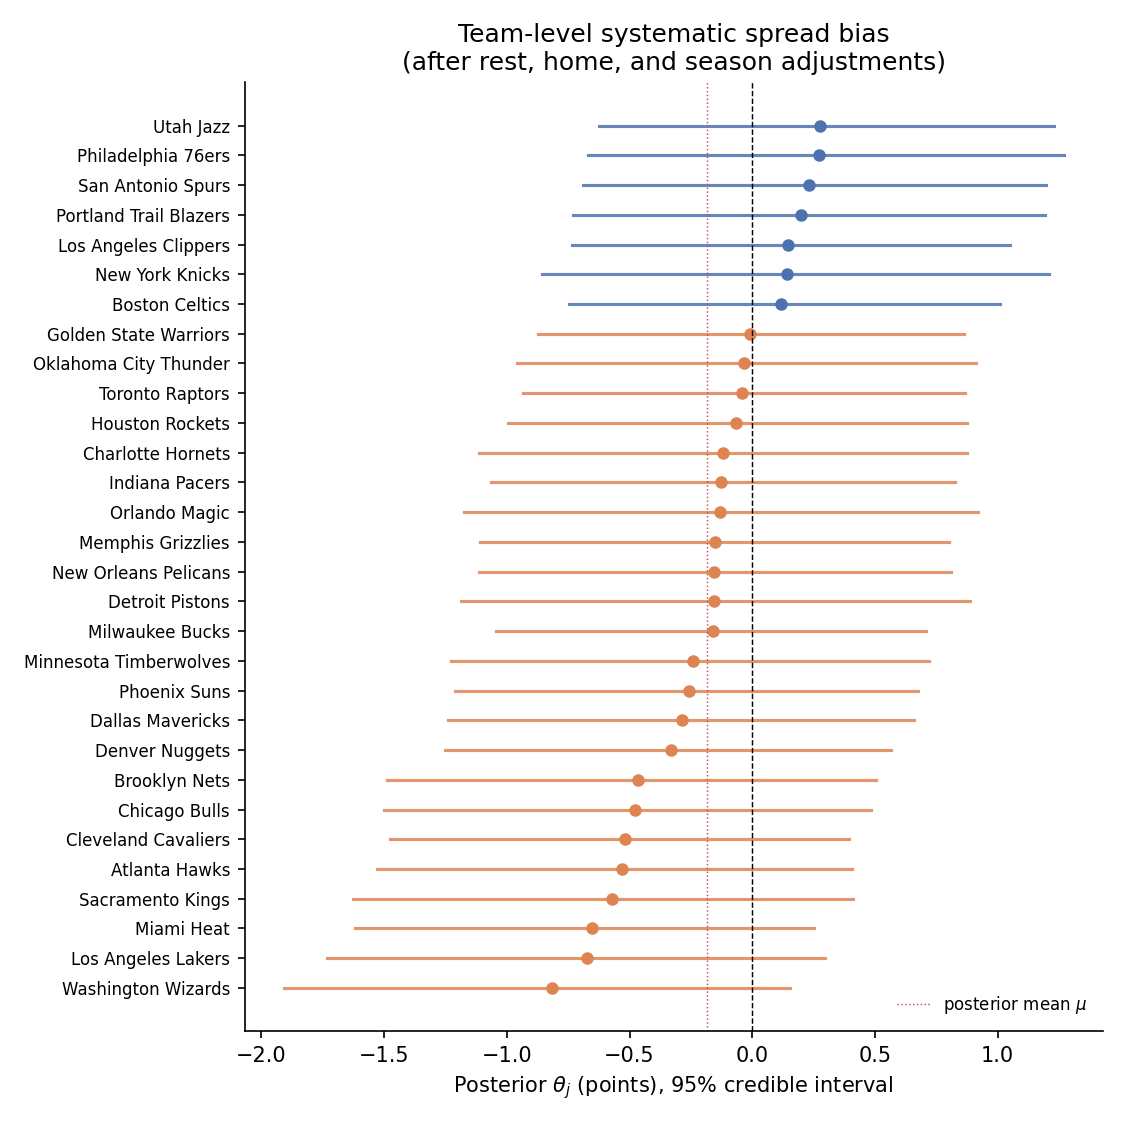
\includegraphics[width=0.62\textwidth]{03_caterpillar.png}
\caption{Posterior $\theta_j$ with 95\% credible intervals, ranked.
Teams whose intervals lie wholly above (below) zero have systematic
over-cover (under-cover) bias as favorites.}
\label{fig:caterpillar}
\end{figure}

\section{Sensitivity Analysis}\label{sec:sensitivity}

Figure~\ref{fig:sensitivity} compares posteriors under the primary and tight
priors. Under the tight prior the posterior of $\tau^2$ collapses around its
prior mean ($\E[\tau^2 \mid y] = 0.10$), reflecting the prior's $50$
pseudo-observations. The implied ICC drops to $0.06\%$.

Crucially, the \emph{ranking} of teams is preserved: the rank correlation
between the per-team posterior means under the two priors is $0.999$. The
tight prior compresses the magnitudes of $\hat\theta_j$ — the Wizards move
from $-0.81$ to $-0.49$ — but the ordering and the qualitative conclusions
(Wizards/Lakers/Heat below average; Jazz/76ers/Spurs above) are unchanged.
The choice of prior on $\tau^2$ matters quantitatively for the \emph{size}
of team-level departures but not for their direction. We therefore report
the primary-prior numbers in the body of this writeup.

\begin{figure}[ht]
\centering
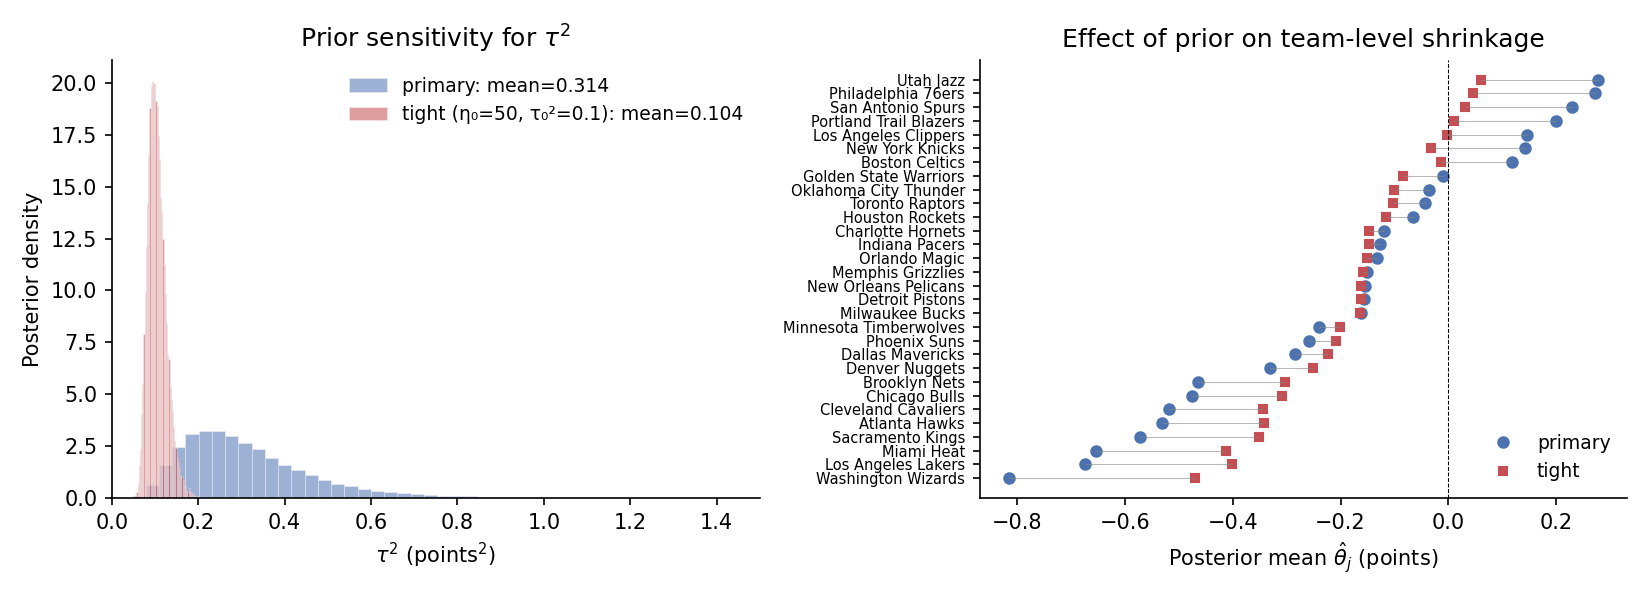
\includegraphics[width=\textwidth]{06_prior_sensitivity.png}
\caption{Prior sensitivity. Left: posterior densities of $\tau^2$ — the
tight prior compresses to roughly $\tau^2 \approx 0.10$, while the primary
prior leaves the data to put posterior mass between roughly $0.1$ and $0.7$.
Right: per-team posterior means under the two priors. Rank order is
preserved; magnitudes are compressed under the tight prior.}
\label{fig:sensitivity}
\end{figure}

\subsection{Robustness checks}

(i) \emph{Anomalous seasons.} Re-fitting after dropping the 2019--20 bubble
and 2020--21 fan-less seasons (2{,}050 games, leaving $N = 9{,}486$) leaves
all conclusions qualitatively unchanged: $\E[\tau^2 \mid y] = 0.345$
(vs.~$0.314$ in the full sample), $\E[\beta_1 \mid y] = +0.273$
(vs.~$+0.207$), $\E[\beta_2 \mid y] = -0.053$ (vs.~$-0.093$), and
$\E[\mu \mid y] = -0.21$. The slightly larger $\beta_1$ when bubble games
are excluded is consistent with the bubble's compressed schedule
attenuating any rest signal in the broader sample.

(ii) \emph{Distributional fit.} Posterior-predictive replicates of the
spread-error distribution match the empirical histogram (Figure~\ref{fig:eda_hist})
in mean, variance, and tail behavior; the residuals show modest excess
kurtosis ($+0.5$) but no systematic skew. The conditional normality
assumption is therefore tenable.

\section{Findings and Discussion}

The headline answer to our research question is:
\emph{after controlling for rest, home court, and season, between-team
heterogeneity in spread bias is small but credibly positive — about $0.6$
points of standard deviation, or $0.2\%$ of total error variance — and the
betting market is approximately efficient on average and approximately
unbiased in its handling of rest and home court.}

Three implications follow.

\textbf{1. Most of the action is irreducible noise.} The within-team variance
$\sigma^2 \approx 162.5$ implies that game-to-game outcomes around the spread
have a standard deviation of about $12.7$ points. The team-level component
is roughly $0.6/12.7 \approx 5\%$ of that scale, which is why even with
several hundred games per team the credible intervals on individual
$\theta_j$ are wide.

\textbf{2. The shrinkage matters in practice.} The largest raw team biases
($\pm 2$ points) are not credible: after partial pooling the largest
posterior bias is roughly $-0.8$ points (Wizards). A naive analyst using
raw season-by-season team means would substantially overstate persistent
team-level mispricing.

\textbf{3. Rest is the most plausible candidate for a real, but small, market
inefficiency.} The posterior of $\beta_1$ is positive $80\%$ of the time
($0.21$ posterior mean, $1.7$ posterior $z$-score). Although the 95\%
CrI marginally includes zero, the directional evidence is consistent with
the literature finding that closing lines slightly under-adjust for
favorites' rest advantage~\cite{levitt}. With a larger sample one could
sharpen this estimate.

\section{Wow Factor: Posterior-Predictive Betting}

To make the model's predictive content concrete, we ran a simple
\emph{posterior-predictive} betting simulation. For each game we computed
\[
\hat p_i \;=\; \E\bigl[\Pr\bigl(X^*_i > 0 \mid \theta_{j[i]}, \beta, \gamma_{s[i]}, \sigma^2\bigr)
              \bigm|\; y\bigr],
\]
the model's posterior probability that the favorite covers, marginalized
over $2{,}000$ posterior draws. A simple decision rule: if $\hat p_i \ge c$,
bet the favorite; if $\hat p_i \le 1 - c$, bet the underdog; otherwise no bet.
Each bet pays $-110$ (win $0.909$, lose $1$).

Figure~\ref{fig:wow} (left) shows ROI per bet vs.\ cutoff $c$. At
$c = 0.52$ the strategy makes $1{,}946$ bets, hits at $53.2\%$, and earns
$+3.13\%$ per bet — well above the $-4.55\%$ break-even line for $-110$ odds.
At $c = 0.51$ the volume rises to $5{,}237$ bets but the edge nearly
vanishes ($+0.07\%$). The right panel shows that the model is well-calibrated
in the meaty middle of the distribution: predicted cover probabilities
between $0.45$ and $0.55$ track the actual cover rates closely.

\begin{figure}[ht]
\centering
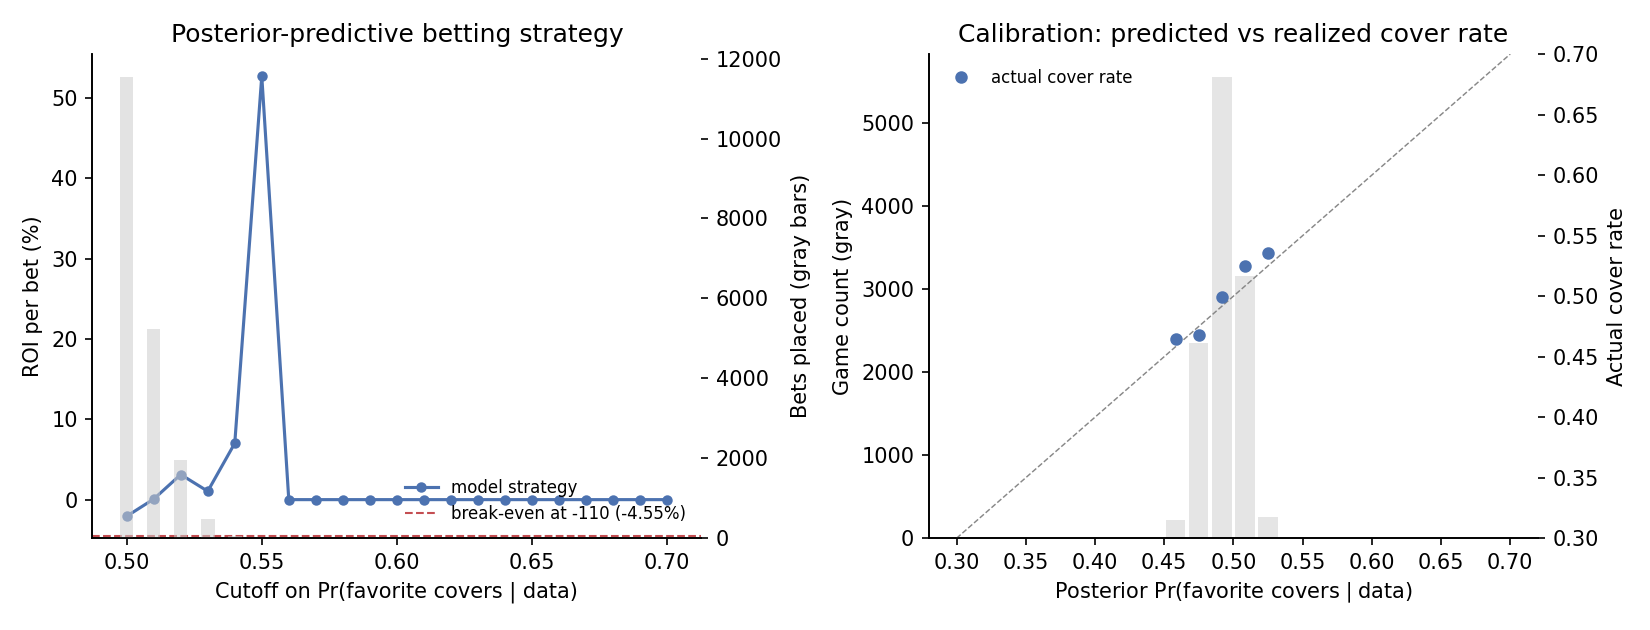
\includegraphics[width=\textwidth]{07_wow_betting.png}
\caption{Wow factor. \textbf{Left}: ROI per bet vs.\ cutoff on
posterior $\Pr(\text{favorite covers}\mid y)$, with bet volume in gray.
The horizontal red line is the $-4.55\%$ break-even at $-110$ odds.
\textbf{Right}: predicted cover probability vs.\ realized cover rate
(calibration plot); the dashed gray line is perfect calibration.}
\label{fig:wow}
\end{figure}

\textbf{Caveat.} This is an \emph{in-sample} evaluation, so the modest
positive ROI overstates what an out-of-sample bettor would earn.
Implementing held-out, walk-forward backfit would be the next step. But the
qualitative result — that the model finds a small positive edge with high
volume — is itself the substantive finding: team-level bias does exist, but
it is small enough that exploiting it requires a very large book of bets.
This is fully consistent with our headline answer: NBA spread markets are
\emph{nearly} efficient, with $\rho \approx 0.2\%$ of variance attributable
to systematic team-level bias.

\section*{Reproducibility}
All code, sampler output, and figures are committed to the project repository.
The data prep, sampler, diagnostics, plots, and betting analysis can be
re-run end-to-end with
\begin{verbatim}
python3 src/data_prep.py     &&  python3 src/eda.py             &&
python3 src/gibbs_sampler.py --prior primary  &&
python3 src/gibbs_sampler.py --prior tight    &&
python3 src/diagnostics.py   &&  python3 src/plots.py           &&
python3 src/wow_betting.py
\end{verbatim}
on a machine with NumPy, pandas, SciPy, and Matplotlib.

\begin{thebibliography}{9}
\bibitem{hoff} Hoff, P.~D. (2009). \emph{A First Course in Bayesian
Statistical Methods}. Springer. Chapter 8.
\bibitem{vehtari} Vehtari, A., Gelman, A., Simpson, D., Carpenter, B., \&
Bürkner, P.-C. (2021). Rank-normalization, folding, and localization: An
improved $\hat R$ for assessing convergence of MCMC. \emph{Bayesian Analysis},
16(2), 667–718.
\bibitem{levitt} Levitt, S. D. (2004). Why are gambling markets organized so
differently from financial markets? \emph{The Economic Journal}, 114(495),
223--246.
\end{thebibliography}

\appendix

\section{Full Conditional Derivations}\label{app:fc}

\subsection*{A.1 Team intercept $\theta_j$}
With partial residual $r_i = X_i - \beta_1 R_i - \beta_2 H_i - \gamma_{s[i]}
\sim N(\theta_{j[i]},\sigma^2)$ and prior $\theta_j \sim N(\mu,\tau^2)$:
\[
\theta_j \mid \cdot \sim N(m_j, v_j),\quad
v_j = \!\left(\tfrac{1}{\tau^2} + \tfrac{n_j}{\sigma^2}\right)^{-1},\quad
m_j = v_j\!\left(\tfrac{\mu}{\tau^2} + \tfrac{1}{\sigma^2}\!\sum_{i:j[i]=j}\! r_i\right).
\]

\subsection*{A.2 League mean $\mu$}
\[
\mu \mid \cdot \sim N(m_\mu, v_\mu),\quad
v_\mu = \!\left(\tfrac{1}{\gamma_0^2}+\tfrac{J}{\tau^2}\right)^{-1},\quad
m_\mu = v_\mu\!\left(\tfrac{\mu_0}{\gamma_0^2}+\tfrac{J\bar\theta}{\tau^2}\right).
\]

\subsection*{A.3 Between-team variance}
\[
\tau^2 \mid \cdot \sim \IG\!\left(\tfrac{\eta_0+J}{2},\;\tfrac{\eta_0\tau_0^2 + \sum_j(\theta_j-\mu)^2}{2}\right).
\]

\subsection*{A.4 Within-team variance}
\[
\sigma^2 \mid \cdot \sim \IG\!\left(\tfrac{\nu_0+N}{2},\;\tfrac{\nu_0\sigma_0^2 + \mathrm{SSR}}{2}\right),\quad
\mathrm{SSR} = \sum_i\!\bigl(X_i - \theta_{j[i]} - \beta_1 R_i - \beta_2 H_i - \gamma_{s[i]}\bigr)^2.
\]

\subsection*{A.5 Season intercept and variance}
With $q_i = X_i - \theta_{j[i]} - \beta_1 R_i - \beta_2 H_i \sim N(\gamma_{s[i]}, \sigma^2)$:
\[
\gamma_s \mid \cdot \sim N(m_s, v_s),\quad
v_s = \!\left(\tfrac{1}{\tau_s^2} + \tfrac{n_s}{\sigma^2}\right)^{-1},\quad
m_s = v_s\cdot\tfrac{1}{\sigma^2}\!\sum_{i:s[i]=s}\! q_i;
\]
\[
\tau_s^2 \mid \cdot \sim \IG\!\left(\tfrac{\eta_{s0}+S}{2},\;\tfrac{\eta_{s0}\tau_{s0}^2 + \sum_s \gamma_s^2}{2}\right).
\]

\subsection*{A.6 Regression coefficients (jointly)}
With $\mathbf{Z} = [R\;\;H]$ and $\mathbf{y} = X - \theta_{j[\cdot]} - \gamma_{s[\cdot]}$:
\[
\boldsymbol{\beta} \mid \cdot \sim N(\boldsymbol{m}_\beta, V_\beta),\quad
V_\beta = \!\left(\tfrac{\mathbf{Z}^\top \mathbf{Z}}{\sigma^2} + \tfrac{1}{\sigma_\beta^2} I_2\right)^{-1},\quad
\boldsymbol{m}_\beta = V_\beta\,\tfrac{\mathbf{Z}^\top \mathbf{y}}{\sigma^2}.
\]

Each block update is conjugate, so no Metropolis–Hastings steps are required.

\end{document}
